\documentclass{ctexrep}
\usepackage{authblk}
\usepackage{amsmath}
\usepackage{amssymb}
\usepackage{amsthm}
\usepackage{hyperref}
\usepackage{algorithm}
\usepackage{algorithmic} 
\renewcommand\equationautorefname{式}
\renewcommand\sectionautorefname{节}
\renewcommand\subsectionautorefname{小节}
\renewcommand\figureautorefname{图}
\newcommand{\algorithmautorefname}{算法}
\bibliographystyle{plain}
\author{姓名\\
	学号\\
	{\small \texttt{\href{mailto:电子邮件地址}{电子邮件地址}}}}
\affil{院系}
\title{《数据仓库与数据挖掘技术》项目报告\\
	报告标题}

\begin{document}

\maketitle
\tableofcontents

\begin{abstract}
	简要介绍一下你的Project所完成的工作,300字以内。\textbf{务必在此处突出说明项目的加分项。}
\end{abstract}

\chapter{主要功能与实现方法(For project 1 \& 2)}

请在这部分说明你的程序主要实现了哪些功能,以及你是通过怎样的原理如何实现的,宜有图例辅助说明。图例请用figure环境,可以这样引用:\autoref{fig-test}。

\section{功能1:……}

\begin{figure}
	\centering
	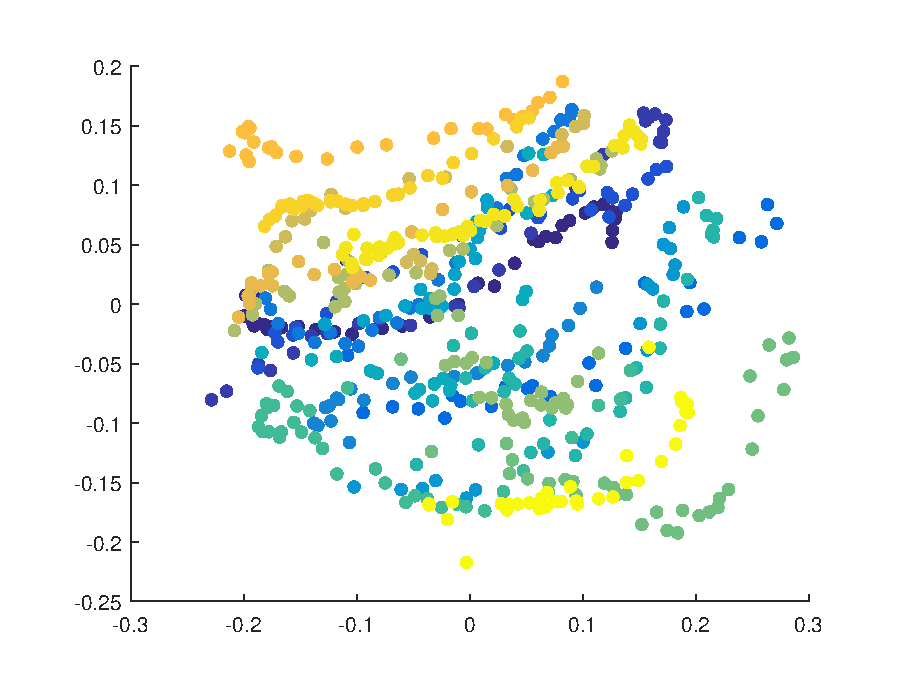
\includegraphics[width=\linewidth]{images/test}
	\caption{这是一个测试图例(这里图片放在images目录下,上面引用时无需扩展名,图片格式可以是jpg,png,eps等)}
	\label{fig-test}
\end{figure}

\section{功能2:……}

\chapter{算法特点与描述(For project 3 \& 4)}

\section{算法特点}

简要介绍这个算法可以用来做什么,和其他算法相比有什么优点。

\section{算法描述}

请对你在本作业中使用的算法原理进行详细的描述,不要Copy\&Paste,宜列出公式和伪代码。有参考文献的话请引用,可以这样引用:\cite{bertsekas2003convex}。把引用的文献信息放在\texttt{references.bib}里。Google Scholar里面选“引用”之后底下有一个BibTeX的选项,把里面的内容复制粘贴到\texttt{references.bib}里就可以了。

\begin{equation}\label{pythagorean}
	c^2 = a^2 + b^2
\end{equation}

上面是一个公式。可以这样引用:\autoref{pythagorean}。

\begin{algorithm}
	\caption{Q-learning迭代算法}
	\label{algorithm-Q-learning}
	\begin{algorithmic}
		\STATE 随机初始化$ Q[num\_states, num\_actions] $
		\STATE 获得初始状态s
		\REPEAT
		\STATE 选择并执行一个动作a
		\STATE 获得奖励r和新状态$ s^{'} $
		\STATE $ Q[s, a] = Q[s, a] + \alpha(r + \gamma \max_{a^{'}}Q[s^{'}, a^{'}] - Q[s, a]) $
		\STATE $ s = s^{'} $
		\UNTIL 终止		
	\end{algorithmic}		
\end{algorithm}	

算法的伪代码可以这样引用:\autoref{algorithm-Q-learning}。

\chapter{实验}

\section{程序运行环境和操作说明}

这里写助教应当如何编译并测试你所提交的程序。

\section{运行结果}

应当包括:程序性能、计算出的结果展示等,宜使用图表进行展示。

\bibliography{references}

\section*{网络资料}

以下是示例。

\begin{itemize}
	\item Quantum Information and Quantum Computation by Wim van Dam \url{https://www.cs.ucsb.edu/~vandam/teaching/S05_CS290/}	
\end{itemize}

\end{document}
